\documentclass[twocolumn,11pt]{article}

\usepackage[margin=2.2cm,columnsep=0.8cm]{geometry}
\usepackage{amsmath,amssymb,bm}
\usepackage{graphicx}
\usepackage{booktabs}
\usepackage{multirow}
\usepackage{caption}
\usepackage{subcaption}
\usepackage{microtype}
\usepackage{tikz}
\usetikzlibrary{arrows.meta,positioning,fit,calc}
\usepackage[colorlinks=true,linkcolor=blue!55!black,citecolor=blue!55!black,urlcolor=blue!55!black]{hyperref}
\usepackage{natbib}
\setcitestyle{authoryear,round,comma,aysep={}}
\usepackage{siunitx}
\sisetup{detect-weight=true, detect-family=true,
         group-minimum-digits=4, group-separator={,}}
\usepackage{xcolor}

\captionsetup{font=small,labelfont=bf}
\setlength{\bibsep}{2pt}
\renewcommand{\topfraction}{0.95}
\renewcommand{\textfraction}{0.05}
\renewcommand{\floatpagefraction}{0.85}
\renewcommand{\dbltopfraction}{0.95}
\renewcommand{\dblfloatpagefraction}{0.85}
\setcounter{dbltopnumber}{3}

% ------------------------------------------------------------------
\title{\bfseries Running an End-to-End Machine-Learning Data Assimilation
System on a Laptop: Porting HealDA to Apple Silicon, Auditing Its
Numerical Trustworthiness, and Ablating GNSS Radio Occultation
Observations}

\author{Anonymous author\thanks{%
Code and data: \url{https://github.com/sonet-hkust/healda-apple-silicon}.
The manuscript was prepared with the assistance of an AI coding agent
(WorkBuddy); all experiments were run on the author's local machine.}}
\date{September 24, 2026}

\begin{document}
\maketitle

\begin{abstract}
Machine-learning (ML) weather models now rival operational numerical
weather prediction (NWP), and end-to-end ML data assimilation (DA)
systems such as HealDA
\citep{gupta2026healda} can map a 24-hour window of observations
directly to a global analysis state in a single forward pass. Yet such
systems are normally evaluated only on data-centre GPUs, and little is
known about (i) whether they can run, reproducibly and trustworthily, on
consumer accelerator hardware, and (ii) how the composition of the
observation stream shapes the resulting analysis. We port HealDA
(327\,M parameters, HEALPix ViT) to an Apple M5 laptop with 32\,GB of
unified memory using the PyTorch Metal Performance Shaders (MPS)
backend, requiring two non-trivial adaptations: a vendored
\texttt{earth2grid} shim for HEALPix indexing, and a patch suite for two
Metal-specific defects---a hard crash in zero-input
\texttt{nn.Linear} layers of the adaLN-Zero conditioning path, and,
more insidiously, silent corruption of large \texttt{int64}
host-to-device copies during observation encoding. We further show that
the corruption is \emph{not} a precision problem (the model runs in
bfloat16 autocast on both CPU and MPS, and fp32 MPS agrees with fp32 CPU
to $7\times10^{-7}$), but a memory-safety defect that only manifests at
full observation scale ($1.1\times10^{7}$ observations) and mimics a
scientific error: without the fix, the zonal wind of the analysis is
essentially decorrelated from ERA5 ($r=-0.01$), while with the fix CPU
and MPS analyses agree to bf16 noise ($z_{500}$ RMSE
$3.9\ \mathrm{m^2\,s^{-2}}$, $r=1.0000$). Using the repaired pipeline
we evaluate analyses against ERA5 over East Asia for
2024-06-01\,00\,UTC: adding AMSU-A/ATMS/MHS radiances
($3.65\times10^{6}$ values) to the conventional stream
($1.13\times10^{7}$ values) reduces layer-mean RMSE by 68\% (temperature),
78\% (geopotential), 36\% (humidity), 36\% (zonal wind) and 20\%
(meridional wind), and removes a $-25$ to $-30$\,gpm zonal-mean bias in
$z_{500}$. A four-way ablation of GNSS radio occultation (RO)
observations---which constitute 71\% of the conventional stream by
count---shows that (a) RO contributes 10--15\% additional RMSE
reduction in temperature, geopotential and humidity over an
RO-free conventional analysis, (b) RO alone matches or exceeds the
full conventional stream in the upper stratosphere (150\,hPa
temperature $r=0.979$ vs.\ $0.974$) but degrades sharply below
500\,hPa, and (c) removing the two background-value channels
(\texttt{gps\_t}, \texttt{gps\_q}) that HealDA ingests alongside
bending angles collapses the meridional-wind skill of an RO-only
analysis from $r=0.44$ to $r=0.05$, demonstrating that the network has
learned a joint $O$--$B$ mapping rather than a pure retrieval. We
discuss the implications for ingesting non-UFS RO data such as
FengYun-3 GNOS into a pretrained HealDA, and for the general practice
of verifying accelerator-ported ML DA systems.
\end{abstract}

\section{Introduction}\label{sec:intro}

The skill of AI weather models has advanced explosively, from
FourCastNet \citep{pathak2022fourcastnet} and Pangu-Weather
\citep{bi2023pangu} to GraphCast \citep{lam2023graphcast} and Aurora
\citep{bodnar2024aurora}, with medium-range skill now comparable to
operational NWP \citep{bauer2015quiet}. Almost all of these systems,
however, still depend on a conventional variational DA system to
provide initial conditions, which ties an otherwise
near-instantaneous forecast pipeline to hours of high-performance
computing. HealDA \citep{gupta2026healda} addresses this with an
encoder--decoder transformer that maps a short window of satellite
and conventional observations directly onto a global $1^{\circ}$
analysis state on the HEALPix sphere \citep{gorski2005healpix},
trained against ERA5 \citep{hersbach2020era5} using replayed UFS
GEFSv13 observations. HealDA analyses initialized off-the-shelf
forecast models (FCN3, Aurora, FengWu) lose less than one day of
effective lead time relative to ERA5-initialized forecasts.

Two aspects of HealDA's ecosystem remain underexplored. First, its
public release has been exercised almost exclusively on CUDA GPUs; the
vendor-locked \texttt{earth2grid} extension shipped as CUDA-12
x86\_64 binaries, and the interaction of its observation encoder with
non-CUDA backends is undocumented. Second, its sensitivity to the
\emph{composition} of the observation stream---which sensors matter,
and how the network represents observation types it was trained
on---is only partially characterized by the end-to-end scores in
\citet{gupta2026healda}. Both questions matter for groups wishing to
re-use HealDA with their own observation sources, for example the
FengYun-3 GNOS radio occultation sounder
\citep{liao2016gnos}, whose data are processed operationally in China
but are not part of the UFS replay stream.

This paper reports a complete, reproducible local deployment of
HealDA on Apple Silicon and uses it to run a series of controlled
observation-subset experiments. Our contributions are:

\begin{enumerate}
\item \textbf{Port.} A minimal, non-invasive adaptation of HealDA to
the PyTorch MPS backend on an Apple M5 (32\,GB unified memory),
including a pure-PyTorch shim for the CUDA-only \texttt{earth2grid}
HEALPix grid, and two \texttt{mps\_patch} modules for Metal-specific
defects (\S\ref{sec:port}). The full conventional-observation analysis
runs in 59\,s (vs.\ 960\,s on CPU) on a laptop.
\item \textbf{Trust audit.} We show that a large CPU--MPS analysis
discrepancy is \emph{not} a floating-point precision issue but a
silent memory-corruption defect in Metal's handling of large
\texttt{non\_blocking} \texttt{int64} copies, we localize it with
layer-wise hook bisection, and we repair it with an input-construction
patch whose correctness we verify down to bf16 noise
(\S\ref{sec:trust}). We document the diagnostic path because the
failure mode---plausible-looking but degraded analyses at scale, with
identical results at toy scale---is a hazard for any backend port of
an ML DA system.
\item \textbf{Observation-subset evaluation.} Against ERA5 over East
Asia, we quantify the analysis impact of (i) satellite radiances
(AMSU-A, ATMS, MHS) on top of the conventional stream and (ii) GNSS
radio occultation observations within it, via a four-way ablation
(all conventional / conventional without RO / RO three-channel /
RO bending-angle only) (\S\ref{sec:sat}, \S\ref{sec:ro}); the RO
ablation is undertaken out of the author's professional interest in
GNSS-RO data assimilation.
\item \textbf{Interpretation.} We clarify the semantics of the RO
channels in the UFS diagnostic stream---the companion \texttt{gps\_t}
and \texttt{gps\_q} channels are \emph{model-background samples at the
bending-angle locations}, not retrievals---and connect the ablation
outcome to the classical 3D-Var formalism
\citep{lorenc1986analysis,courtier1994strategy,daley1991atmospheric}
and to the known prior-contamination issue of 1D-Var retrieval
assimilation (\S\ref{sec:interpretation}).
\end{enumerate}

All code, figure-generation scripts, per-level verification statistics
and the compiled manuscript are publicly available\footnote{%
\url{https://github.com/sonet-hkust/healda-apple-silicon}}.

\section{The HealDA system and data}\label{sec:system}

\subsection{Architecture}
HealDA \citep{gupta2026healda} is an observation encoder followed by a
HEALPix vision transformer (a DiT-L adaptation with 24 blocks, width
1024, 327.2\,M parameters). The encoder buckets observations by sensor
family into fixed-size token grids; each (pixel, bucket) cell is
aggregated with a masked scatter-mean so that absent sensors are
explicitly flagged through an observability mask. The trunk operates
on $12288$ tokens (HPX64 grid, $n_{\mathrm{side}}=64$, $49152$ cells
at $\approx0.92^{\circ}$, $2\times2$ patchification), and the decoder
emits 74 output channels: five dynamical fields (temperature $T$,
zonal and meridional wind $u,v$, geopotential $z$, specific humidity
$q$) on 13 pressure levels (1000, 925, 850, 700, 600, 500, 400, 300,
250, 200, 150, 100, 50\,hPa) plus nine surface variables. The release
checkpoint (\texttt{healda\_ufs\_era5.mdlus}, 1.22\,GB) carries five
observation embedders: \texttt{conv} (8 conventional channels
$\times$ 33-wide tokens $=$ 264 bins) and four radiance buckets
(AMSU-A 120 platform-channel bins, ATMS 44, MHS 25, AMSU-B).
Conditioning is unconditional in the released configuration; the
adaLN-Zero modulation layers are therefore
\texttt{nn.Linear(0, 6144)}---a detail that becomes important in
\S\ref{sec:port}. Inference is a single forward pass over the
24-hour observation window $[t_0-21\mathrm{h},\,t_0+3\mathrm{h}]$.

\subsection{Observation stream}
We use the NOAA UFS GEFSv13 replay observations served by
\texttt{earth2studio} \citep{earth2studio} for
2024-06-01\,00\,UTC. Table~\ref{tab:obs} inventories the stream. Two
facts deserve emphasis. First, RO bending angles and their two
companion channels constitute $8.04\times10^{6}$ of the
$1.134\times10^{7}$ conventional values (71\%); HealDA's conventional
bucket is dominated, by count, by GNSS RO. Second, the RO companion
channels \texttt{gps\_t} and \texttt{gps\_q} are not retrievals:
in the UFS/GSI diagnostic convention they are the
\emph{model first-guess temperature and specific humidity sampled at
the bending-angle report locations}, while the BUFR 1D-Var retrieval
fields (descriptors 12001/13001) are deliberately not exported. We
return to the implications in \S\ref{sec:interpretation}.

\begin{table}[t]
\centering
\caption{Observation inventory for 2024-06-01\,00\,UTC
(window $[t_0-21\mathrm{h},t_0+3\mathrm{h}]$, UFS GEFSv13 replay).
``RO'' = GNSS radio occultation; ``bkg.''\ marks background (first
guess) values sampled at the report locations.}
\label{tab:obs}
\small
\begin{tabular}{@{}llr@{}}
\toprule
Group & Channel & Count \\
\midrule
\multirow{3}{*}{RO} & \texttt{gps} (bending angle $\alpha$) & \num{2680664} \\
 & \texttt{gps\_t} (bkg.\ $T$) & \num{2680664} \\
 & \texttt{gps\_q} (bkg.\ $q$) & \num{2680664} \\
\midrule
\multirow{4}{*}{In-situ} & $u$ & \num{1080489} \\
 & $v$ & \num{1080489} \\
 & $T$ & \num{617321} \\
 & surface $p$ & \num{428354} \\
 & $q$ & \num{91356} \\
\midrule
\multicolumn{2}{l}{Conventional subtotal} & \num{11340001} \\
\midrule
\multirow{3}{*}{Radiance} & AMSU-A & \num{2136601} \\
 & ATMS & \num{985798} \\
 & MHS & \num{528756} \\
\midrule
\multicolumn{2}{l}{Satellite subtotal} & \num{3651155} \\
\bottomrule
\end{tabular}
\end{table}

The reported bending angles have median $8.96\times10^{-4}$\,rad,
median tangent pressure 30.4\,hPa, and geographic coverage to
$\pm79^{\circ}$ latitude, consistent with the limb-sounding geometry
of GNSS RO \citep{kursinski1997observing,anthes2008cosmic}.
Figure~\ref{fig:obscomp} visualizes the inventory on a logarithmic
count axis; the dominance of the three RO channels is immediate.

\begin{figure}[t]
\centering

\includegraphics[width=\columnwidth]{figures/fig10_obs_composition.pdf}
\caption{Observation composition of the 2024-06-01\,00\,UTC stream
(counts of Table~\ref{tab:obs}, logarithmic axis). The three GNSS-RO
channels dominate the conventional bucket, and AMSU-A dominates the
radiance suite.}
\label{fig:obscomp}
\end{figure}

\subsection{Verification data}
Analyses are verified against the ERA5 pressure-level reanalysis
\citep{hersbach2020era5} valid at the same time, interpolated from a
$0.25^{\circ}$ regional extract (93--127$^{\circ}$E,
16--43$^{\circ}$N; East Asia) onto the common 13-level set. HealDA
fields are sampled from the native HEALPix grid onto the ERA5 grid by
Delaunay linear interpolation with nearest-neighbour infill. We report
RMSE, the Pearson correlation $r$ with ERA5, and the ratio of
spatial standard deviations (a sharpness indicator). A single case
study cannot establish climatological significance; its value is
process-level attribution under fully controlled input subsets,
enabled by the fact that a HealDA analysis is a deterministic
function of its observation vector.

\section{Porting HealDA to Apple Silicon}\label{sec:port}

\subsection{Environment}
The host is an Apple M5 laptop with 32\,GB unified memory running
macOS. The software stack is Python 3.12.12 (managed by
\texttt{uv}), PyTorch 2.10.0 with the MPS backend, and the NVIDIA
\texttt{earth2studio} 0.18.0 / \texttt{physicsnemo} 2.2.2 releases
with \texttt{timm} 1.0.30 and \texttt{makani} 0.2.0. No CUDA
components are installed.

\subsection{The \texttt{earth2grid} shim}
HealDA's input pipeline indexes observation locations onto the HEALPix
grid through NVIDIA's \texttt{earth2grid} package, whose official
distribution ships CUDA-12 x86\_64 binaries and therefore cannot be
installed on Apple Silicon. The HEALPix functionality actually
required by the released checkpoint is narrow: an \texttt{ang2pix}
mapping from (longitude, latitude) to pixel index under the padded
XY pixel ordering, plus grid lat/lon attributes. We vendor a
$\sim$100-line pure-PyTorch shim implementing this subset, validated
to reproduce the reference pixel indexing. The shim is built
on demand by a small \texttt{build\_shim.py} utility and inserted at
the front of \texttt{sys.path}; the upstream package is never
modified.

\subsection{Metal defect 1: zero-input \texttt{nn.Linear}}
Because the released HealDA is an unconditional regressor, the
adaLN-Zero modulation layers are degenerate
\texttt{nn.Linear} instances with \texttt{in\_features = 0} (25 of
them: 24 blocks plus the detokenizer). On MPS, a forward pass through
such a layer aborts the process inside
\texttt{MPSNDArray initWithDevice:\ldots} with
\texttt{Error: device may not be nil} (SIGABRT without a Python
traceback); merely moving the layer to Metal is harmless, only the
forward crashes.

The repair exploits the fact that with zero inputs the layer is a
\emph{constant function}:
\begin{equation}
y = xW^{\top} + b = b ,
\end{equation}
so evaluating it anywhere is exact. \texttt{patch\_for\_mps()}
replaces each such layer with a CPU-pinned stub whose
\texttt{\_apply} is a no-op (so a later \texttt{.to("mps")} cannot
drag the weights onto Metal) and whose forward simply returns the
stored bias. Output equality with the original layer is bit-exact
(max $|\Delta| = 0.00$ over the full analysis run).

\subsection{Metal defect 2: silent corruption of large
\texttt{int64} copies}
The second defect produces no crash, no warning and no Python-level
error---it silently degrades the science. It is the subject of the
next section.

\section{A numerical trust audit of the MPS backend}\label{sec:trust}

\subsection{Symptom}
The first MPS analyses (2024-06-01\,00\,UTC, full conventional
stream) verified far worse against ERA5 than a CPU reference run of
the same configuration: layer-mean $r$ of meridional wind was
$-0.01$ (i.e.\ uncorrelated), zonal wind 0.45, and temperature 0.75,
versus 0.88, 0.94 and 0.95 on CPU (Table~\ref{tab:layers}). Initial
suspicion fell on reduced-precision arithmetic.

\subsection{The precision hypothesis is false}
Precision was ruled out by direct measurement:
\begin{itemize}
\item The inference script hard-codes bfloat16 autocast on
\emph{both} devices
(\texttt{torch.autocast(self.device.type, dtype=torch.bfloat16)});
the CPU reference was never an fp32 golden run. With the autocast
op-routing conventions verified identical on CPU and MPS (matmuls and
linear layers in bf16; softmax, layernorm and reductions in fp32),
a 24-layer LayerNorm-plus-residual chain at width 1024 diverges from
an fp32 reference by $4.81\times10^{-3}$ on CPU and
$4.81\times10^{-3}$ on MPS---indistinguishable---while MPS fp32
agrees with CPU fp32 to $7.2\times10^{-7}$.
\item The masked scatter-mean aggregation
(\texttt{scatter\_reduce\_} with \texttt{reduce="mean"}) is
\emph{bit-identical} between CPU and MPS at every occupancy tested
(2--1000 observations per cell, 0.00e+00 difference), in both fp32
and bf16.
\item The 25 CPU-pinned stubs of \S\ref{sec:port} return exactly the
original biases (max $|\Delta| = 0.00$).
\end{itemize}
Notably, a 20\,000-observation subsample produced
\emph{bit-consistent} encoder outputs between devices
(relative $\ell_2 = 8.6\times10^{-7}$): the defect scales with
observation count, the signature of a resource-management bug rather
than arithmetic.

\subsection{Localization}
Registering forward hooks on every stage of the observation encoder
and bisecting the CPU--MPS divergence localized the corruption to the
input-construction routine \texttt{build\_input()}, \emph{before} any
network computation: of its outputs, \texttt{obs}, \texttt{pix},
\texttt{obs\_type} and \texttt{offsets} matched CPU exactly, while
the metadata tensor was already garbage on MPS. A targeted re-check
identified the corrupted tensor:

\begin{quote}\small
\texttt{target\_time} (shape $[1.01\times10^{7}]$, \texttt{int64}):\\
CPU: \texttt{1717200000, 1717200000, \ldots} (epoch seconds, correct)\\
MPS: \texttt{1717124400000000000, \ldots} (observed times in
nanoseconds)
\end{quote}

\texttt{build\_input()} assembles its tensors column-by-column with
\texttt{.to("mps", non\_blocking=True)}. Under Metal, the later
copies in this sequence overwrite earlier buffers---a buffer-lifetime
/ aliasing defect in the host-to-device copy path---so the
\texttt{target\_time} column arrives corrupted with values belonging
to a different column. Downstream, the relative-time feature
computes $\Delta t = (\texttt{target\_time}\times10^{9} -
t_{\mathrm{obs}})$, which overflows \texttt{int64} and yields
$10^{8}$-second garbage; the encoder is then fed wrong timing
information for every observation. Calling
\texttt{torch.mps.synchronize()} does not repair it, and a minimal
isolated reproducer with a single \texttt{non\_blocking} copy does
not trigger it, indicating sensitivity to the specific multi-column
copy sequence rather than to any single call.

\subsection{Repair and verification}
The fix, \texttt{patch\_build\_input\_on\_cpu()}, temporarily swaps
\texttt{model.device\_buffer} for an empty CPU tensor so that
\texttt{model.device} reports CPU and \texttt{build\_input()}
constructs its tensors entirely in host memory; the completed
dictionary is then moved to the accelerator with synchronous copies.
Observation encoding becomes device-consistent
(relative $\ell_2 = 1.99\times10^{-2}$, $r = 0.99979$ vs.\ CPU; the
residual is bf16 noise), and the analysis is restored
(Table~\ref{tab:layers}, Figs.~\ref{fig:mpsmaps}--\ref{fig:mpsscatter}).
Two further checks support stability: two independent MPS runs differ
by less than CPU and MPS differ (0.015\,K vs.\ 0.033\,K layer-mean
temperature RMSE), i.e.\ no stochastic corruption remains; and the
conventional+satellite run reproduces the same behaviour
(406\,s, 10.5\,GB peak).

\begin{figure*}[t]
\centering

\includegraphics[width=\textwidth]{figures/fig1_mps_failure.pdf}
\caption{850\,hPa temperature over East Asia for 2024-06-01\,00\,UTC.
Top: ERA5 truth and the CPU reference analysis. Bottom: the MPS
analysis before and after the input-construction repair. Before the
repair the MPS analysis is smoothly biased (RMSE 6.11\,K,
$r=0.663$); after the repair it matches the CPU reference
(RMSE 2.15\,K vs.\ 2.12\,K, $r=0.924$ vs.\ $0.926$).}
\label{fig:mpsmaps}
\end{figure*}

\begin{figure}[t]
\centering
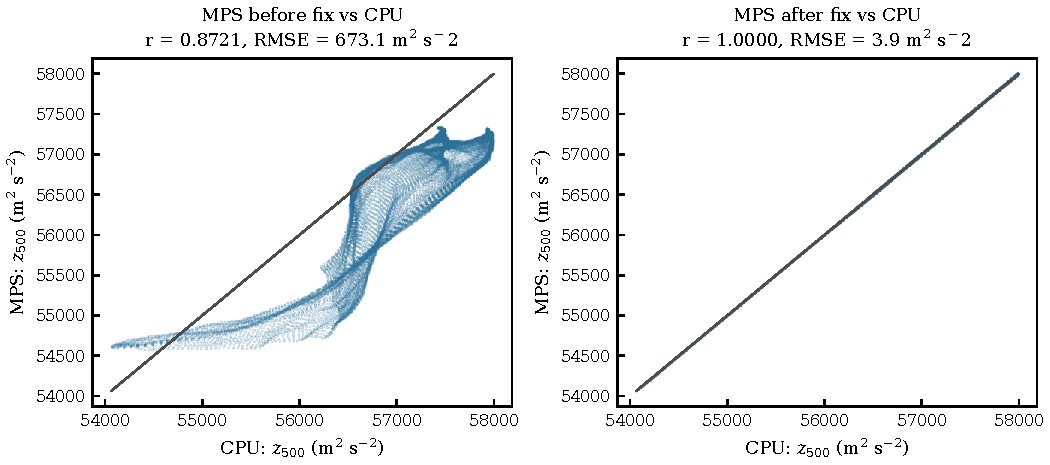
\includegraphics[width=\columnwidth]{figures/fig2_mps_scatter.pdf}
\caption{500\,hPa geopotential, MPS vs.\ CPU reference, over all
verification points. Left: before the repair ($r=0.872$,
RMSE $673\ \mathrm{m^2\,s^{-2}}$). Right: after the repair
($r=1.0000$, RMSE $3.9\ \mathrm{m^2\,s^{-2}}$, consistent with bf16
noise).}
\label{fig:mpsscatter}
\end{figure}

\begin{table*}[t]
\centering
\caption{Layer-mean verification against ERA5 over East Asia
(13 levels, 2024-06-01\,00\,UTC). RMSE in
$\mathrm{K}$ ($T$), $\mathrm{m\,s^{-1}}$ ($u,v$),
$\mathrm{m^2\,s^{-2}}$ ($z$) and
$\mathrm{mg\,kg^{-1}}$ ($q$); $r$ = spatial correlation;
SR = standard-deviation ratio.}
\label{tab:layers}
\footnotesize
\setlength{\tabcolsep}{5pt}
\begin{tabular}{@{}l cc cc cc cc cc@{}}
\toprule
 & \multicolumn{2}{c}{$T$} & \multicolumn{2}{c}{$u$} &
   \multicolumn{2}{c}{$v$} & \multicolumn{2}{c}{$z$} &
   \multicolumn{2}{c}{$q$} \\
\cmidrule(lr){2-3}\cmidrule(lr){4-5}\cmidrule(lr){6-7}\cmidrule(lr){8-9}\cmidrule(lr){10-11}
Experiment & RMSE & $r$ & RMSE & $r$ & RMSE & $r$ & RMSE & $r$ & RMSE & $r$ \\
\midrule
CPU reference (bf16)      & 2.50 & 0.946 & 3.03 & 0.943 & 2.42 & 0.880 & 611 & 0.960 & 592 & 0.844 \\
MPS before repair         & 5.00 & 0.749 & 8.76 & 0.454 & 7.48 & $-0.011$ & 1431 & 0.746 & 2155 & 0.323 \\
MPS after repair (conv)   & 2.50 & 0.946 & 3.04 & 0.943 & 2.41 & 0.881 & 612 & 0.960 & 590 & 0.844 \\
Conventional + satellite  & \textbf{0.80} & \textbf{0.983} & \textbf{1.96} & \textbf{0.967} & \textbf{1.92} & \textbf{0.907} & \textbf{135} & \textbf{0.993} & \textbf{378} & \textbf{0.923} \\
\bottomrule
\end{tabular}
\end{table*}

\begin{table}[t]
\centering
\caption{Cost of a single 2024-06-01\,00\,UTC analysis on the M5
laptop (32\,GB unified memory).}
\label{tab:cost}
\footnotesize
\begin{tabular}{@{}lccc@{}}
\toprule
Configuration & Device & Wall time & Peak memory \\
\midrule
Conventional      & CPU & 960\,s & 16.0\,GB \\
Conventional      & MPS & 59\,s  & 8.6\,GB \\
Conv.\ + satellite & MPS & 406\,s & 10.5\,GB \\
\bottomrule
\end{tabular}
\end{table}

\section{Conventional versus conventional-plus-satellite}\label{sec:sat}

With the repaired pipeline we quantify the analysis impact of
microwave radiances by comparing the conventional-only analysis with
one that additionally ingests $3.65\times10^{6}$ AMSU-A/ATMS/MHS
radiance values (Table~\ref{tab:layers},
Figs.~\ref{fig:satprofile}--\ref{fig:satzonal}).

\textbf{Radiance impact is large across the column.} Layer-mean RMSE
falls by 68\% for temperature (2.50 to 0.80\,K), 78\% for geopotential
(612 to 135\,\si{m^2 s^-2}), 36\% for specific humidity, 36\% for
zonal wind and 20\% for meridional wind; correlations rise to 0.98--0.99
for $T$ and $z$ everywhere below 100\,hPa. At 850\,hPa, temperature
RMSE drops from 2.15 to 0.74\,K and $r$ from 0.924 to 0.981.

\textbf{The largest gains are tropical.} In the horizontal
(Fig.~\ref{fig:satspatial}), the conventional analysis shows its worst
temperature and geopotential errors in the 16--25$^{\circ}$N monsoon
region (up to 6\,K at 850\,hPa, $-600\ \mathrm{m^2\,s^{-2}}$ at
500\,hPa), where the conventional network is sparse; these are nearly
eliminated by the radiances. Mid-latitude wind error changes little,
and isolated small patches degrade slightly---consistent with the
radiance-suite weighting being optimized (at training time) for
global rather than regional skill.

\textbf{The increment itself is positive and broad-scale.}
Figure~\ref{fig:incmap} shows the raw analysis increment,
conv+sat $-$ conv, at 500\,hPa. Both temperature and geopotential
increments are positive almost everywhere over East Asia, with
$z_{500}$ lifted by roughly $100$--$400\ \mathrm{m^2\,s^{-2}}$
($\approx$10--40\,gpm) across the domain---the signature of the
radiances pulling the analysis upward toward ERA5, consistent with
the bias removal quantified next.

\begin{figure*}[t]
\centering

\includegraphics[width=\textwidth]{figures/fig12_increment_map.pdf}
\caption{Direct analysis increment of adding satellite radiances
(conv+sat $-$ conv) at 500\,hPa over East Asia: temperature (left,
K) and geopotential (right, $\mathrm{m^2\,s^{-2}}$). The increment is
positive nearly everywhere, lifting the mass field toward ERA5.}
\label{fig:incmap}
\end{figure*}

\textbf{The mass-field bias is removed.} The conventional analysis
carries a zonal-mean $z_{500}$ bias of $-25$ to $-30$\,gpm across
15--43$^{\circ}$N (Fig.~\ref{fig:satzonal}); with radiances the bias
is within $-8$ to $-5$\,gpm. We caution that a single-window ML DA
system has no cycling background: part of this bias is attributable
to the absence of a dynamical background rather than to the missing
observations, and the radiance increment should be read as the
envelope of both effects.

\begin{figure*}[t]
\centering

\includegraphics[width=\textwidth]{figures/fig3_profile_sat.pdf}
\caption{Vertical profiles of verification statistics against ERA5
(East Asia, 13 levels): RMSE (top) and spatial correlation (bottom)
for the conventional-only and conventional-plus-satellite analyses.}
\label{fig:satprofile}
\end{figure*}

\begin{figure*}[t]
\centering

\includegraphics[width=\textwidth]{figures/fig4_spatial_sat.pdf}
\caption{Analysis-minus-ERA5 differences for 850\,hPa temperature
(left) and 500\,hPa geopotential (right), conventional-only (top)
versus conventional-plus-satellite (bottom).}
\label{fig:satspatial}
\end{figure*}

\begin{figure}[t]
\centering

\includegraphics[width=\columnwidth]{figures/fig5_improvement_sat.pdf}
\caption{RMSE reduction (in absolute units) from adding satellite
radiances, 850\,hPa temperature (left) and 500\,hPa geopotential
(right). Blue: RMSE reduced; red: RMSE increased.}
\label{fig:satimprove}
\end{figure}

\begin{figure}[t]
\centering

\includegraphics[width=0.82\columnwidth]{figures/fig8_zonal_z500.pdf}
\caption{Zonal-mean 500\,hPa geopotential height (gpm): ERA5 versus
the conventional-only and conventional-plus-satellite analyses.}
\label{fig:satzonal}
\end{figure}

\section{Ablation of GNSS radio occultation observations}\label{sec:ro}

\subsection{Design}
Within the conventional bucket we ran a four-way ablation, enabled by
the per-(pixel, bucket) observability masks with which HealDA encodes
``this sensor family is absent here'':
\begin{enumerate}
\item \textbf{Conv (all)}: the full conventional stream
($1.134\times10^{7}$ values, 71\% of them RO-related);
\item \textbf{Conv w/o RO}: the same stream with the three RO
channels removed (\texttt{--conv-vars pres q t u v});
\item \textbf{RO 3-channel}: bending angles plus their background
$T$/$q$ companions only (\texttt{gps gps\_t gps\_q});
\item \textbf{RO bending-angle only}: \texttt{gps} alone.
\end{enumerate}
All four analyses use the repaired MPS pipeline and are verified
identically.

\subsection{Results}
Table~\ref{tab:ro} summarizes layer-mean statistics;
Figs.~\ref{fig:roprofile} and \ref{fig:rospatial} show vertical and
horizontal structure.

\begin{table*}[t]
\centering
\caption{GNSS-RO ablation: layer-mean verification against ERA5 (13
levels, East Asia). The ``RO impact'' column is the layer-mean RMSE
reduction of \emph{Conv (all)} relative to \emph{Conv w/o RO}.}
\label{tab:ro}
\footnotesize
\setlength{\tabcolsep}{5pt}
\begin{tabular}{@{}l cc cc cc cc cc c@{}}
\toprule
 & \multicolumn{2}{c}{$T$} & \multicolumn{2}{c}{$u$} &
   \multicolumn{2}{c}{$v$} & \multicolumn{2}{c}{$z$} &
   \multicolumn{2}{c}{$q$} \\
\cmidrule(lr){2-3}\cmidrule(lr){4-5}\cmidrule(lr){6-7}\cmidrule(lr){8-9}\cmidrule(lr){10-11}
Experiment & RMSE & $r$ & RMSE & $r$ & RMSE & $r$ & RMSE & $r$ & RMSE & $r$ \\
\midrule
Conv (all)      & 2.50 & 0.946 & 3.04 & 0.943 & 2.41 & 0.881 & 612 & 0.960 & 590 & 0.844 \\
Conv w/o RO     & 2.78 & 0.932 & 3.20 & 0.938 & 2.55 & 0.864 & 697 & 0.962 & 695 & 0.825 \\
RO 3-channel    & 3.95 & 0.898 & 5.03 & 0.748 & 5.40 & 0.441 & 1144 & 0.858 & 1119 & 0.737 \\
RO bangle only  & 5.56 & 0.707 & 9.90 & 0.333 & 6.37 & 0.051 & 1528 & 0.704 & 1950 & 0.575 \\
\midrule
RO impact (RMSE) & $-10.2\%$ & & $-4.9\%$ & & $-5.2\%$ & & $-12.3\%$ & & $-15.1\%$ & \\
\bottomrule
\end{tabular}
\end{table*}

\begin{figure}[t]
\centering

\includegraphics[width=0.82\columnwidth]{figures/fig9_zonal_bias_z500.pdf}
\caption{Zonal-mean $z_{500}$ bias against ERA5 for the ablation
experiments (plus the conventional-plus-satellite analysis for
context).}
\label{fig:robias}
\end{figure}

\begin{figure*}[t]
\centering

\includegraphics[width=\textwidth]{figures/fig6_profile_ro.pdf}
\caption{As Fig.~\ref{fig:satprofile}, for the RO ablation
experiments.}
\label{fig:roprofile}
\end{figure*}

\begin{figure*}[t]
\centering

\includegraphics[width=\textwidth]{figures/fig11_ro_cross_section.pdf}
\caption{Temperature analysis-minus-ERA5 cross-sections at
110$^{\circ}$E for the four RO-ablation experiments. The
bending-angle-only analysis (right) develops a large cold bias below
100\,hPa, while the RO three-channel analysis remains structurally
close to the full conventional stream in the upper troposphere and
lower stratosphere.}
\label{fig:roxs}
\end{figure*}

\begin{figure*}[t]
\centering

\includegraphics[width=\textwidth]{figures/fig7_spatial_ro.pdf}
\caption{Analysis-minus-ERA5 temperature differences at 300\,hPa
(left) and 850\,hPa (right) for the four ablation experiments.}
\label{fig:rospatial}
\end{figure*}

\textbf{RO contributes 10--15\% to the conventional analysis in
mass, temperature and humidity, and little in wind.} Removing RO
degrades layer-mean RMSE by 10.2\% ($T$), 12.3\% ($z$) and 15.1\%
($q$), but only 4.9--5.2\% ($u,v$). This is the expected physics:
bending angles constrain temperature and geopotential directly
(through refractivity and hydrostatic balance) but influence winds
only indirectly through geostrophic adjustment, mirroring the
experience of variational RO assimilation
\citep{cucurull2008utilization,healy2006assimilation}. The zonal-mean
mass-field signature of the ablation is shown in
Fig.~\ref{fig:robias}: the $-25$ to $-30$\,gpm bias of the full
conventional analysis is barely changed by removing RO (noRO), but
grows monotonically as the observation set is reduced to RO-only
variants.

\textbf{RO alone is competitive in the upper stratosphere and weak in
the lower troposphere.} At 150\,hPa the RO-only (3-channel)
temperature correlation, 0.979, exceeds the full conventional
analysis (0.974); at 100\,hPa it matches it (0.9689 vs.\ 0.9690)
with a \emph{lower} RMSE (3.34 vs.\ 4.37\,K). Below 500\,hPa the
RO-only analysis degrades rapidly (850\,hPa $T$: $r=0.843$ vs.\
0.924; Fig.~\ref{fig:roprofile}), reproducing the classical
``strong above, weak below'' vertical signature of RO
\citep{anthes2008cosmic,healy2006assimilation} within an ML DA
system. Notably, the bending-angle-only analysis has the \emph{lowest}
100\,hPa temperature RMSE of all experiments (2.40\,K) but the lowest
standard-deviation ratio (0.73), i.e.\ a locally accurate but
over-smoothed field---a reminder that RMSE alone can hide the loss of
variance in a regression toward the mean. The same structure is
visible in the latitude--height cross-sections of
Fig.~\ref{fig:roxs}: the cold bias that fills the troposphere of the
bending-angle-only analysis and the near-neutral full column of the
three-channel analysis, in contrast to the structured, smaller-magnitude
bias field of the full conventional stream.

\textbf{Background companions carry decisive information.} Dropping
\texttt{gps\_t}/\texttt{gps\_q} from the RO-only analysis collapses
layer-mean $v$ from $r=0.441$ to $r=0.051$ (uncorrelated), $T$ from
0.898 to 0.707, and $z$ from 0.858 to 0.704. The network has not been
trained to retrieve the atmosphere from bending angles; it has been
trained to map the \emph{pair} (observation, background) to an
analysis. We interpret this next.

\section{Interpretation: RO channels as $(O, B)$ pairs}\label{sec:interpretation}

In 3D-Var the RO analysis problem is
\begin{multline}\label{eq:3dvar}
J = \tfrac{1}{2}\,(x - x_b)^{\top} B^{-1}(x - x_b)\\
  + \tfrac{1}{2}\,\bigl(H(x) - y_o\bigr)^{\top} R^{-1}
      \bigl(H(x) - y_o\bigr),
\end{multline}
with increment $\delta x = BH^{\top}(HBH^{\top}+R)^{-1}d$ and
innovation $d = y_o - H(x_b)$ \citep{lorenc1986analysis,
daley1991atmospheric, courtier1994strategy}. The background enters
\emph{twice}: as the prior centre of the first term, and inside
$H(x_b)$ in the innovation. The three RO channels of the UFS
diagnostic stream correspond exactly to the pieces of this machinery
that a learned operator must be fed explicitly:

\begin{center}
\small
\begin{tabular}{@{}lll@{}}
\toprule
Channel & 3D-Var analogue & Status \\
\midrule
\texttt{gps}    & $y_o$ (bending angle) & observation \\
\texttt{gps\_t} & $H(x_b)$, $T$ part    & background \\
\texttt{gps\_q} & $H(x_b)$, $q$ part    & background \\
\bottomrule
\end{tabular}
\end{center}

HealDA does not implement a bending-angle forward operator $H$; it
receives $H(x_b)$ directly (GSI diagnostics must store it to compute
$O-B$ anyway) and learns the combined map
$(y_o, x_b|_{\mathrm{obs}})\!\rightarrow\!x_a$, i.e.\ the roles that
$B$, $R$, $H^{\ast}$ (adjoint) and the innovation computation play in
\eqref{eq:3dvar} are absorbed into the network weights. Three
observations support this reading. First, the collapse experiment:
without the $B$ channels the RO-only analysis degenerates
(\S\ref{sec:ro}), because the network has never seen bending angles
unanchored by a background. Second, the geometry: a bending angle is
a non-local Abel transform of the refractivity profile,
$\alpha(a) = -2a\int_a^{\infty} \frac{\mathrm{d}\ln n}{\mathrm{d}x}
\frac{\mathrm{d}x}{\sqrt{x^2-a^{2}}}$, whereas the network consumes
un-ordered scatter points that carry no profile identity---inverting
the Abel integral from such a representation without a local anchor
is severely ill-posed, which is exactly what the $r=0.05$ meridional
wind exhibits. Third, the observation-space semantics: the two
background channels are kept separate from the (identical-unit)
regular $T$ and $q$ channels---their normalization statistics differ
by about 20\,K in the mean, reflecting the stratosphere-weighted
RO report distribution---and the released checkpoint's own
normalization file documents them as a distinct measurement method.

This design has an underappreciated advantage over the alternative
operational pathway of assimilating 1D-Var retrievals: in retrieval
assimilation the background used inside the retrieval leaks into the
``observation'' and is then counted again in \eqref{eq:3dvar}
through the prior term, a double-counting that biases analyses
toward the background and is a classical reason the community
converged on bending-angle assimilation
\citep{cucurull2008utilization,healy2006assimilation}. HealDA keeps
the observation and the prior in separate, explicit channels---no
prior is baked into the observation---so the information bookkeeping
is cleaner. The cost is symmetrical: the influence of the background
is frozen into the trained weights, with no external $B$-variance
dial to turn, and the model is only valid for background statistics
from its training system.

\section{Practical implications}\label{sec:implications}

\paragraph{For accelerator porting.} The MPS defect documented here
produces \emph{plausible but degraded} analyses and is invisible to
smoke tests: at $2\times10^{4}$ observations the encoder output is
bit-consistent across devices. The general lesson for porting ML DA
systems is that parity testing must be performed at production
observation scale, on every input tensor of the data pipeline (not
only the model), and against field-level truth, because an ML DA
system degrades gracefully and therefore hides memory-safety bugs.
The two patches presented here are each about twenty lines and make
no change to the model or its weights; they are generic enough to be
reusable for other physicsnemo DiT models on Metal.

\paragraph{For re-using HealDA with new observation sources.}
The checkpoint's observation embedders are frozen: the bucket
membership (five families) and bin counts are hard-coded in the
trained weights, so \emph{adding} a sensor family requires training a
new embedder; \emph{subsetting} existing families, however, is natively
supported through the observability masks, as our ablation
demonstrates. For a group wishing to feed, e.g., FengYun-3 GNOS
bending angles \citep{liao2016gnos} into the released checkpoint, the
practical path is the \texttt{conv} bucket's \texttt{gps} slots,
with two hard requirements: (i) the companion background $T$/$q$
values must be provided from a background consistent with the
training system's climatology, since the ablation shows they carry
decisive information; and (ii) the bending-angle normalization
(training mean \num{0.00411}\,rad, standard deviation
\num{0.00602}\,rad) must be applied unchanged. Vertical coverage is
additionally bounded by the training data (RO reports to 0.5\,hPa in
the UFS stream); systematically truncated profiles constitute an
out-of-distribution sparsity pattern that the observability masks
will flag but cannot correct.

\paragraph{For laptop-scale DA experiments.} The repaired MPS
pipeline completes the conventional-only analysis in 59\,s
(8.6\,GB peak) and the conventional-plus-satellite analysis in
406\,s (10.5\,GB peak) on a fanless-class laptop
(Table~\ref{tab:cost}), against 960\,s and 16.0\,GB on CPU. This
makes controlled ablation ensembles of the kind in
\S\ref{sec:ro} an interactive rather than batch activity, and puts a
single-window global analysis within reach of classroom-scale
hardware.

\section{Conclusions}\label{sec:conclusions}

We ported the HealDA ML data assimilation system to Apple Silicon,
diagnosed and repaired a silent memory-corruption defect that had
previously been misattributed to reduced-precision arithmetic, and
used the repaired pipeline to quantify, in a controlled single-case
setting, the analysis impact of microwave radiances and of GNSS
radio occultation observations over East Asia. The principal
findings are that (i) satellite radiances dominate the analysis
quality, reducing layer-mean RMSE by 20--78\% depending on the
variable and largely removing a zonal-mean mass-field bias; (ii) RO
observations, although 71\% of the conventional stream by count,
contribute a further 10--15\% RMSE reduction concentrated in
temperature, geopotential and humidity, with RO-only skill matching
the full conventional stream in the upper stratosphere; and (iii)
the RO analysis skill depends jointly on the bending angles and
their background-value companion channels, consistent with a learned
$(O,B)\!\rightarrow\!x_a$ map rather than a retrieval, and
illustrating how a trained network internalizes the roles of $B$,
$R$ and the adjoint of a variational system.

Limitations. Our verification is a single case (2024-06-01\,00\,UTC)
over East Asia against ERA5, which is itself the training target of
HealDA; neither sampling uncertainty nor the verification-target
relationship is addressed, and the RMSE gaps reported here should be
read as process-level attribution rather than climatological skill
estimates. The MPS repair is validated to bf16 noise, not to fp32,
and the Metal defect itself is upstream of our code. Extending the
ablation to multiple dates, to the satellite bucket, and to
observation-system experiments with real FengYun-3 GNOS profiles is
the natural continuation.

\appendix

\section{Reproducing the experiments}\label{app:repro}

The repository layout is
\texttt{code/} (pipeline scripts), \texttt{paper/} (this manuscript,
figure script and statistics) and \texttt{analysis\_outputs/}
(regional gridded analyses in CF-1.8 NetCDF, openable with
\texttt{ncview}). Environment: Python 3.12, PyTorch 2.10,
\texttt{earth2studio} 0.18.0, \texttt{physicsnemo} 2.2.2
(\texttt{uv} lock file included). The HealDA checkpoint
(\texttt{healda\_ufs\_era5.mdlus}) is fetched automatically by
\texttt{earth2studio} on first use. Each experiment in this paper is
a single invocation of the analysis driver with a date, a device
(\texttt{--device cpu} or \texttt{--device mps}), an output path, and
a sensor selection: \texttt{--sensors conv} for the conventional
stream, \texttt{--sensors both} to add microwave radiances, and
\texttt{--conv-vars} to restrict the conventional bucket to an
arbitrary subset of its eight channels (e.g.\ the three RO channels
alone, or the conventional stream with RO removed)---the switch that
enables the ablations of \S\ref{sec:ro}.

The \texttt{--device mps} path applies both patches of
\S\ref{sec:port} automatically. Native HEALPix outputs are converted
to regular lat-lon CF-1.8 files by
\texttt{code/06\_to\_latlon.py} (cKDTree $k=6$ Gaussian-weighted
regridding, $0.55^{\circ}$ effective smoothing) and verified by
\texttt{paper/make\_figures.py}, which recomputes every statistic and
figure in this manuscript from the NetCDF files. Note that the
verification figures use direct Delaunay interpolation of the native
grid (no smoothing), which is the statistically conservative choice;
the smoothed regridding is provided for visualization.

\section{Per-level verification statistics}\label{app:stats}

The complete per-level table (7 experiments $\times$ 5 variables
$\times$ 13 levels, with RMSE, bias, correlation and
standard-deviation ratio against ERA5) is machine-readable at
\texttt{paper/stats.csv} and \texttt{paper/stats.json} in the
repository. Figure~\ref{fig:roprofile} and
Figure~\ref{fig:satprofile} display the same data graphically.

\section*{Data and code availability}
All scripts (analysis driver, MPS patches, HEALPix shim, regridding
and figure generation), the per-level verification statistics
(\texttt{stats.csv}), and this manuscript are available at
\url{https://github.com/sonet-hkust/healda-apple-silicon}. The
HealDA checkpoint is distributed with \texttt{earth2studio}; ERA5
data were obtained from the Copernicus Climate Data Store.

\section*{Acknowledgements}
The HealDA system was developed by NVIDIA, NOAA and MITRE
\citep{gupta2026healda}; we thank the authors for the public
release of the checkpoint and of \texttt{earth2studio}. This study
used the UFS GEFSv13 replay observation stream distributed through
\texttt{earth2studio} and ERA5 from the Copernicus Climate Change
Service.

\bigskip
\noindent\fbox{\parbox{0.97\columnwidth}{\small
This work, including all experiments, data analysis and the writing
of this report, was completed with the support of
\textbf{hy4-preview-f}. Readers interested in this study are welcome
to contact the author at \texttt{xhubw@connect.ust.hk}.}}

\begin{thebibliography}{99}\small

\bibitem[Gupta et al.(2026)]{gupta2026healda}
Gupta, A., A. Subramaniam, M. S. Pritchard, K. Kashinath,
S. Frolov, K. Lieberman, C. Miller, N. Silverman, and
N. D. Brenowitz, 2026: HealDA: Highlighting the importance of
initial errors in end-to-end AI weather forecasts.
\emph{arXiv preprint arXiv:2601.17636}.
\bibitem[Hersbach et al.(2020)]{hersbach2020era5}
Hersbach, H., and co-authors, 2020: The ERA5 global reanalysis.
\emph{Q.\ J.\ R.\ Meteorol.\ Soc.}, \textbf{146}, 1999--2049.
\bibitem[G\'orski et al.(2005)]{gorski2005healpix}
G\'orski, K. M., E. Hivon, A. J. Banday, B. D. Wandelt,
F. K. Hansen, M. Reinecke, and M. Bartelmann, 2005: HEALPix: A
framework for high-resolution discretization and fast analysis of
data distributed on the sphere. \emph{Ap.\ J.}, \textbf{622},
759--771.
\bibitem[Pathak et al.(2022)]{pathak2022fourcastnet}
Pathak, J., and co-authors, 2022: FourCastNet: A global data-driven
high-resolution weather model using adaptive Fourier neural operators.
\emph{arXiv preprint arXiv:2202.11214}.
\bibitem[Bi et al.(2023)]{bi2023pangu}
Bi, K., and co-authors, 2023: Accurate medium-range global weather
forecasting with 3D neural networks. \emph{Nature}, \textbf{619},
533--538.
\bibitem[Lam et al.(2023)]{lam2023graphcast}
Lam, R., and co-authors, 2023: Learning skillful medium-range global
weather forecasting. \emph{Science}, \textbf{382}, 1416--1421.
\bibitem[Bodnar et al.(2024)]{bodnar2024aurora}
Bodnar, C., and co-authors, 2024: Aurora: A foundation model for the
Earth system. \emph{arXiv preprint arXiv:2405.13063}.
\bibitem[Bauer et al.(2015)]{bauer2015quiet}
Bauer, P., A. Thorpe, and G. Brunet, 2015: The quiet revolution of
numerical weather prediction. \emph{Nature}, \textbf{525}, 47--55.
\bibitem[Lorenc(1986)]{lorenc1986analysis}
Lorenc, A. C., 1986: Analysis methods for numerical weather
prediction. \emph{Q.\ J.\ R.\ Meteorol.\ Soc.}, \textbf{112},
1177--1194.
\bibitem[Courtier et al.(1994)]{courtier1994strategy}
Courtier, P., J.-N. Th\'epaut, and A. Hollingsworth, 1994: A strategy
for operational implementation of 4D-Var, using an incremental
approach. \emph{Q.\ J.\ R.\ Meteorol.\ Soc.}, \textbf{120},
1367--1387.
\bibitem[Daley(1991)]{daley1991atmospheric}
Daley, R., 1991: \emph{Atmospheric Data Analysis}. Cambridge
University Press, 457 pp.
\bibitem[Kursinski et al.(1997)]{kursinski1997observing}
Kursinski, E. R., G. A. Hajj, J. T. Schofield, R. P. Linfield, and
K. R. Hardy, 1997: Observing Earth's atmosphere with radio
occultation measurements using the Global Positioning System.
\emph{J.\ Geophys.\ Res.}, \textbf{102}, 23429--23465.
\bibitem[Anthes et al.(2008)]{anthes2008cosmic}
Anthes, R. A., and co-authors, 2008: The COSMIC/FORMOSAT-3 mission:
Early results. \emph{Bull.\ Am.\ Meteorol.\ Soc.}, \textbf{89},
313--333.
\bibitem[Cucurull et al.(2008)]{cucurull2008utilization}
Cucurull, L., J. C. Derber, R. Treadon, and R. J. Purser, 2008:
Assimilation of GPS radio occultation observations into NCEP's
Global Data Assimilation System. \emph{Mon.\ Wea.\ Rev.},
\textbf{136}, 2777--2796.
\bibitem[Healy and Th\'epaut(2006)]{healy2006assimilation}
Healy, S. B., and J.-N. Th\'epaut, 2006: Assimilation experiments
with CHAMP GPS radio occultation measurements. \emph{Q.\ J.\ R.\
Meteorol.\ Soc.}, \textbf{132}, 605--623.
\bibitem[Liao et al.(2016)]{liao2016gnos}
Liao, M., P. Zhang, G.-L. Yang, Y.-M. Bi, Y. Liu, W.-H. Bai,
X.-G. Meng, Q.-F. Du, and Y.-Q. Sun, 2016: Preliminary validation of
the refractivity from the new radio occultation sounder GNOS/FY-3C.
\emph{Atmos.\ Meas.\ Tech.}, \textbf{9}, 781--792.
\bibitem[Paszke et al.(2019)]{paszke2019pytorch}
Paszke, A., and co-authors, 2019: PyTorch: An imperative style,
high-performance deep learning library. \emph{Advances in Neural
Information Processing Systems 32}.
\bibitem[Micikevicius et al.(2018)]{micikevicius2018mixed}
Micikevicius, P., and co-authors, 2018: Mixed precision training.
\emph{arXiv preprint arXiv:1710.03740}.
\bibitem[NVIDIA(2025)]{earth2studio}
NVIDIA, 2025: Earth2Studio: A framework for AI weather and climate
prediction workflows. \emph{Software}, v0.18.0,
\url{https://github.com/NVIDIA/earth2studio}.

\end{thebibliography}

\end{document}
